% =====================================================================
% IEEE Robotics and Automation Letters (RA-L) submission draft.
% Single file: macros, figures (pgfplots), tables and bibliography.
% Limit: 6 pages + up to 2 over-length pages (8 total, references included).
%
% \tbd{} marks a result still to run. Every finished number is re-derived
% from results/octvla_results.tar.xz; see paper/numbers_provenance.md.
% Before submission: grep for \tbd and VERIFY, which must both be gone.
% =====================================================================
\documentclass[letterpaper, 10pt, journal, twoside]{IEEEtran}

\usepackage{cite}
\usepackage{amsmath,amssymb}
\usepackage{graphicx}
\usepackage{booktabs,multirow}
\usepackage{xcolor}
\usepackage{pgfplots}
\pgfplotsset{compat=1.17}
\usepackage[hidelinks]{hyperref}

% Placeholder for a result not yet run. Red so that none survives unnoticed.
\newcommand{\tbd}[1][]{\textcolor{red}{\textbf{xx}#1}}
\newcommand{\arm}[1]{\texttt{#1}}
\newcommand{\figbox}[2]{%
  \fbox{\parbox[c][#1][c]{0.95\linewidth}{\centering\footnotesize\textit{#2}}}}

\markboth{IEEE Robotics and Automation Letters. Preprint Version. Accepted Month, Year}
{Younes \MakeLowercase{\textit{et al.}}: Objects as Conditions}

\begin{document}

\title{Objects as Conditions: Object-Centric State and Relational
Composition for Pretrained Vision-Language-Action Policies}

\author{Ali~Younes$^{1}$, \textcolor{red}{Co-Author}$^{1}$,
and~\textcolor{red}{Supervisor}$^{1}$%
\thanks{Manuscript received: Month, Day, Year; Revised Month, Day, Year;
Accepted Month, Day, Year.}%
\thanks{This paper was recommended for publication by Editor
\textcolor{red}{Name} upon evaluation of the Associate Editor and Reviewers'
comments.}%
\thanks{\textcolor{red}{Funding acknowledgement.}}%
\thanks{$^{1}$\textcolor{red}{Affiliation, address, e-mail.}}%
\thanks{Digital Object Identifier (DOI): see top of this page.}%
}

\maketitle

% =====================================================================
\begin{abstract}
Pretrained vision-language-action (VLA) policies perceive a manipulation
scene only through pixels. We study whether conditioning them on an explicit
object-centric state helps: an unordered set of entities, each with pose,
size and type. We also study whether the way the entities are composed
matters.

Every conditioned policy is compared against an RGB policy given the same
additional training, over three training seeds. On a dual-arm, multi-object
restocking task, zero-initialised per-entity attention raises the task
success of GR00T~N1.7 from 9 to 35 of 60 scenes with seen objects, and from
0 to 11 of 60 with object sizes held out of training. Under an unseen visual
appearance the RGB policy collapses while the conditioned policy keeps most
of its success.

Two controls locate the gain. Training the identical network on another
scene's entities removes it, so the gain is object information rather than
capacity. A pooled scene vector alone does not reproduce it, so it depends
on each action query retrieving the entities.

The benefit depends on the policy. ACT gains only on held-out sizes, and
pi0.5 and SmolVLA gain nothing once the added capacity is matched.

Building on the retrieval finding, we add a lightweight relational
composition module that passes pairwise relative geometry between entities
before injection. It changes success by \tbd{} on the restocking task and by
\tbd{} on average across five RoboTwin~2.0 tasks. Trained on three objects,
conditioned GR00T policies transfer strongly to two objects and partially to
four, where the relational module reaches \tbd{} of 60.
\end{abstract}

\begin{IEEEkeywords}
Imitation Learning, Deep Learning in Grasping and Manipulation, Bimanual
Manipulation, Representation Learning.
\end{IEEEkeywords}

% =====================================================================
\section{Introduction}
\label{sec:intro}

\IEEEPARstart{M}{ulti-object} manipulation requires a policy to know which
object to act on, where that object is, and where it is relative to
everything else. Vision-language-action (VLA) policies
\cite{bjorck2025gr00t,pi05,shukor2025smolvla} acquire broad visuomotor priors
from large-scale pretraining. When adapted to a new task, however, they must
recover object identity and relative geometry from pixels, from a few dozen
demonstrations. A natural remedy is to tell the policy where the objects are.
ControlVLA~\cite{li2025controlvla} injects object features into a pretrained
policy through zero-initialised key-value attention and reports large gains
in the few-shot regime.

Three questions are open. First, \emph{does object-centric state help once
the extra training it brings is controlled for?} Fine-tuning a conditioned
policy on top of an RGB checkpoint also trains it for longer. We find that
this alone accounts for much of the apparent gain on some backbones. Second,
\emph{which injection carries the benefit?} Per-entity attention, a pooled
scene vector and in-context entity tokens each make different assumptions
about how the objects should be composed. Third, \emph{does composing the
entities relationally help further, and does it help across object counts?}
Many manipulation goals are relations (on top of, inside, left of) rather
than properties of single objects.

We answer these questions with a controlled study on four policy families
(ACT~\cite{zhao2023act}, GR00T~N1.7~\cite{bjorck2025gr00t},
$\pi_{0.5}$~\cite{pi05} and SmolVLA~\cite{shukor2025smolvla}). We use a
dual-arm, multi-object restocking task with held-out object geometry and
varying object count, and five multi-object tasks from
RoboTwin~2.0~\cite{chen2025robotwin2}. Every conditioned arm is paired,
episode by episode, against an RGB control trained for the same number of
additional steps, over three training seeds.

\noindent Our contributions are:
\begin{enumerate}
  \item A budget-controlled comparison of object-centric conditioning
    across four policy families, which shows that the benefit depends on
    the backbone. GR00T improves on seen and held-out objects, ACT only on
    held-out geometry, and $\pi_{0.5}$ and SmolVLA not at all at matched
    capacity (Sec.~\ref{sec:rq1}).
  \item Controls that attribute the GR00T gain to object \emph{information}
    rather than capacity, and to \emph{query-dependent} per-entity retrieval
    rather than a pooled scene summary. We also characterise its robustness
    to pose noise, missing entities and visual shift (Sec.~\ref{sec:rq1}).
  \item A relational composition module and a colour channel, both
    initialised so that training starts from the RGB policy, evaluated with
    matched information and capacity controls (Sec.~\ref{sec:rq2}).
  \item An evaluation of generalisation across object count (train on 3,
    test on 2 and 4) for every conditioning mechanism (Sec.~\ref{sec:rq3}).
\end{enumerate}

\begin{figure}[t]
  \centering
  \figbox{4.2cm}{Teaser. Left: restock scene with the entity set overlaid
  (objects, grippers, shelf decks). Right: filmstrips of the RGB control
  (knocks the object) and \arm{kv} (completes the transfer) on the same
  scene.}
  \caption{Object-centric conditioning of a pretrained VLA. The scene is
  given to the policy as an unordered set of entities. Each action query
  attends to the entities through zero-initialised key-value projections.}
  \label{fig:teaser}
\end{figure}

% =====================================================================
\section{Related Work}
\label{sec:related}

\textbf{Pretrained robot policies.}
ACT~\cite{zhao2023act} predicts action chunks with a transformer trained from
scratch on demonstrations. GR00T~N1~\cite{bjorck2025gr00t} and
$\pi_{0.5}$~\cite{pi05} pair a pretrained vision-language backbone with a
flow-matching action expert. SmolVLA~\cite{shukor2025smolvla} is a compact
variant of this design. All are adapted to new tasks from RGB and
proprioception. Our concern is what explicit object state adds to that
adaptation, and we measure it against a control given the same extra
training, a control rarely reported.

\textbf{Object-centric policies.}
Object-centric representations have long been used to structure visuomotor
learning, from object proposals as priors for imitation~\cite{zhu2022viola}
to unsupervised slot decompositions~\cite{locatello2020slot}.
ControlVLA~\cite{li2025controlvla} adapts pretrained VLAs with object
features through a zero-initialised attention branch. It shows that skipping
RGB pretraining fails, which we replicate. LPWM~\cite{lpwm} conditions a
particle dynamics model on context through adaptive normalisation or tokens,
which motivates two of our injection variants. Unlike these works, we hold
the object representation fixed and vary the injection and the composition,
against a budget-matched control.

\textbf{Relational inductive biases.}
Relation networks~\cite{santoro2017rn} and graph
networks~\cite{battaglia2018relational} compute functions of object pairs.
Set functions~\cite{zaheer2017deepsets} make such computations independent
of entity order and count. We use the simplest relational layer of this kind
that leaves the pretrained policy's behaviour unchanged at initialisation.

% =====================================================================
\section{Method}
\label{sec:method}

\subsection{The entity set}
\label{sec:entities}
A scene is an unordered set of at most $N{=}16$ entities: the movable
objects, both grippers and the support surfaces. A mask marks which rows are
real. Entity $i$ is
$z_i = (p_i, r_i, s_i, a_i, \tau_i) \in \mathbb{R}^{17}$:
\begin{itemize}
  \item $p_i\in\mathbb{R}^3$ is the position in the workcell frame;
  \item $r_i\in\mathbb{R}^6$ is the 6D rotation (two columns of $R_i$);
  \item $s_i\in\mathbb{R}^3$ is the size;
  \item $a_i$ is the gripper aperture (zero for non-grippers);
  \item $\tau_i$ is a one-hot type over \{object, left gripper, right
    gripper, support\}.
\end{itemize}
The set carries no task role, target identity or object identifier, so the
policy is not told which object to move next. Position and size are
standardised with statistics fitted on the training split only. The
continuous and categorical columns are projected separately, summed and
normalised into an embedding $e_i = E(z_i)$. Padded rows are zeroed and
masked out of every attention.

Entities are read from the simulator. We treat them as an upper bound on
what a perception system could supply, and quantify sensitivity to pose
noise and missing entities in Sec.~\ref{sec:robustness}.

\subsection{Two-stage adaptation}
Following ControlVLA~\cite{li2025controlvla}, adaptation has two stages.
\textit{Stage~1} trains the stock policy on RGB and proprioception.
\textit{Stage~2} loads the stage-1 checkpoint and adds a conditioning branch,
initialised so that the stage-2 policy is numerically identical to the
stage-1 policy at the first step. We verify this identity before every
stage-2 run, together with a check that gradient reaches the new branch.

\subsection{Injection mechanisms}
\label{sec:injection}

\textbf{Per-entity attention (\arm{kv}).} In every hooked attention layer of
the host, with query $Q$, keys and values $K,V$ and output projection $W_o$,
the output becomes
\begin{equation}
  W_o\!\left[\mathrm{sm}\!\left(\tfrac{QK^\top}{\sqrt d}\right)V +
  \mathrm{sm}\!\left(\tfrac{QK_z^\top}{\sqrt d}\right)V_z\right],
  \label{eq:kv}
\end{equation}
where $K_z{=}W_k h$ and $V_z{=}W_v h$, with $W_k,W_v$ initialised to zero and
$h_i{=}e_i$. The branch reuses the host's own query and output projection,
so each action query retrieves the entities that are relevant to it. No
positional code is used, because the entities form a set.

\textbf{Scene modulation (\arm{kv\_adaln}).} In addition to \arm{kv}, an
attention pool with one learned query summarises the set into a scene vector
$c$. That vector modulates every block through a zero-initialised adaptive
normalisation, in the style of DiT and LPWM~\cite{lpwm}. In hosts that
already condition their blocks on a vector (GR00T's timestep embedding,
$\pi_{0.5}$'s adaptive RMSNorm), $c$ is added to that vector.

\textbf{Entity tokens (\arm{kv\_tokens}).} In addition to \arm{kv}, the
entities join the host's token sequence behind a learned logit gate
(initialised at $-4$) and are removed before the action read-out. GR00T's
action transformer accepts no attention mask, so the gate cannot be applied
there and this arm is not used on GR00T.

\subsection{Relational composition}
\label{sec:method-rel}
\arm{kv} lets each action query retrieve entities, but each entity embedding
describes one object in absolute coordinates. The relations that define
most multi-object goals, such as which object is above, inside or
left of another and how far the gripper is from each object, must then be
assembled inside the host. The relational arm \arm{kv\_rel} computes them
explicitly, replacing $h_i{=}e_i$ in~\eqref{eq:kv} with a relation-aware
embedding. For every ordered pair of real entities, it expresses $j$ in the
frame of $i$:
\begin{equation}
  u_{ij} = \big[R_i^\top(p_j-p_i),\; \mathrm{6D}(R_i^\top R_j),\;
  \lVert p_j-p_i\rVert,\; s_j-s_i\big],
\end{equation}
and aggregates messages over the other real entities $\mathcal N_i$:
\begin{equation}
  h_i = e_i + W_0\,\frac{1}{|\mathcal N_i|}\sum_{j\in\mathcal N_i}
  \phi\big(e_i,\, e_j,\, \psi(u_{ij})\big),
  \label{eq:rel}
\end{equation}
with $\phi,\psi$ two-layer MLPs.

Three properties follow from this design.
\begin{itemize}
  \item The output does not depend on the order of the entities.
  \item The mean keeps the scale of the message independent of the number
    of entities, which is what generalisation across object count requires.
  \item Gripper-anchored terms ($i\in$ grippers) give the policy the
    gripper-to-object offset directly, instead of the difference of two
    absolute poses.
\end{itemize}
Because $W_k,W_v$ start at zero, \arm{kv\_rel} is identical to stage~1 at
initialisation whatever $W_0$ is. We therefore initialise $W_0$ randomly:
zero-initialising it as well would leave $\phi$ and $\psi$ without gradient
until $W_v$ moves. One message-passing layer is used, and two layers are
evaluated as an ablation. With $N{=}16$, computing all pairs adds
\tbd{}\,M parameters and negligible time.

\subsection{Colour channel}
\label{sec:method-colour}
Two of our RoboTwin tasks define their goal by colour (stack red, then
green, then blue), which no geometric entity can express. The \arm{+c}
variants append each entity's base colour (three columns, zero for grippers
and supports), declared per task. A colour-defined goal therefore tests
whether the conditioning branch can use non-geometric attributes, and
whether geometry alone is inert there.

% =====================================================================
\section{Experimental Setup}
\label{sec:setup}

\subsection{Tasks}

\textbf{Shelf restock.} A dual-arm Franka Panda in SAPIEN moves three boxes
from a lower to an upper shelf deck.
The boxes are drawn from seven sizes that define three identity tiers:
\begin{itemize}
  \item \emph{seen}: sizes 1--4;
  \item \emph{held-out}: sizes 0 and 6, collected but excluded from
    training;
  \item \emph{novel}: size 5, which the oracle has never collected.
\end{itemize}
Demonstrations come from a motion-planning oracle: 75 training runs (31.8k
frames) and 23 validation runs. Policies observe a head camera, two wrist
cameras and proprioception, and output absolute end-effector poses with a
binary gripper command.

Evaluation also varies the number of objects. With two objects, the layout
is a three-object layout with one later object removed, so that the first
target is placed exactly as in training. Four objects stay within the
training workspace. A transfer counts when an object rests on the upper deck
at the end of the episode.

\textbf{RoboTwin~2.0.} We use five multi-object tasks
(Table~\ref{tab:robotwin}). Each comes with RoboTwin's scripted expert and
success check. We collect \tbd{} demonstrations per task with
\tbd[ embodiment] and record entities through the same pipeline as for
restock. Because an expert can fail silently after a planning failure, a
demonstration is kept only if every planned motion succeeded.

\begin{table}[t]
\centering
\caption{RoboTwin~2.0 tasks and the relation each goal requires.}
\label{tab:robotwin}
\footnotesize
\setlength{\tabcolsep}{3pt}
\begin{tabular}{@{}lllc@{}}
\toprule
Task & Movable entities & Goal relation & Colour \\
\midrule
Stack Blocks Three   & 3 blocks          & stacked R/G/B          & \checkmark \\
Blocks Ranking RGB   & 3 blocks          & ordered R, G, B in $x$ & \checkmark \\
Put Bottles Dustbin  & 3 bottles, bin    & containment, sequence  & -- \\
Place Cans Plasticbox & 2 cans, box      & bimanual containment   & -- \\
Place Bread Basket   & 2 breads, basket  & containment            & -- \\
\bottomrule
\end{tabular}
\end{table}

\subsection{Policies and training}

\textbf{ACT.} Trained from scratch for 40k steps per stage at batch 8, with
chunk 50.

\textbf{GR00T~N1.7.} Frozen vision-language backbone. The action head is
trained for 8k steps per stage at batch 16.

\textbf{$\pi_{0.5}$ and SmolVLA.} Frozen VLM, with LoRA of rank 32 on every
projection of the action expert, for 8k steps per stage at batch 16. For
these two backbones the object branch is low-rank, so that it adds 8--19\% of
trainable parameters, close to GR00T's +9\%. The default LeRobot LoRA would
make the branch 40--120$\times$ larger than everything else being trained,
and any gain would be confounded with capacity.

\textbf{Execution.} All policies execute 25 actions per inference call.

\subsection{Arms, controls and statistics}

\textbf{Controls.} The \emph{budget control} \arm{rgb\_cont} continues
stage~1 for exactly the steps that stage~2 adds. Every conditioned arm is
compared against it, not against stage~1. \arm{scratch\_kv} trains \arm{kv}
without stage~1.

\textbf{Evaluation.} Each cell is trained with three seeds. Each seed is
evaluated on the same 20 pinned scenes per tier and per object count. The
simulator verifies the requested object sizes on every reset. Episodes last
600 steps with three objects and 200 steps per object otherwise. We report:
\begin{itemize}
  \item task success;
  \item the number of episodes with at least one transfer;
  \item stage-wise survival.
\end{itemize}

\textbf{Statistics.} Arms are compared with a two-sided exact McNemar test
on matched (training seed, scene) episodes. Because many contrasts are
tested, we treat $p<0.05$ as a lead and make a claim only when the effect
has the same sign on every training seed. Validation loss is never used to
select checkpoints: in this setting it contradicted closed-loop success
repeatedly, so every cell is scored from its final checkpoint.

\textbf{Training format.} Demonstrations are used as continuous runs rather
than per-object clips. In a paired study from one set of oracle executions,
policies trained on per-object clips almost never chained a second transfer
(2 of 26 attempts, against 9 of 24). Continuous runs raised three-object
success from 1 to 9 of 60 ($p=0.008$) and two-object success from 3 to 19
($p<0.001$).

% =====================================================================
\section{RQ1: Is Object-Centric State Useful?}
\label{sec:rq1}

\begin{table*}[t]
\centering
\caption{Restock, three objects. Successes and episodes with $\geq$1
transfer, out of 60 (3 training seeds $\times$ 20 scenes), each paired
against the budget control \arm{rgb\_cont} of the same backbone (exact
McNemar $p$ in parentheses). Bold: $p<0.05$ with the same sign on every
training seed.}
\label{tab:rq1}
\footnotesize
\begin{tabular}{@{}llcccc@{}}
\toprule
Backbone & Arm & Success, seen & Success, held-out & $\geq$1 transfer, seen & $\geq$1 transfer, held-out \\
\midrule
\multirow{5}{*}{ACT}
 & \arm{rgb\_cont}  & 21 & 0 & 39 & 15 \\
 & \arm{kv}         & 22 (1.00) & 0 (--) & 37 (0.85) & 17 (0.82) \\
 & \arm{kv\_adaln}  & 22 (1.00) & \textbf{7 (0.016)} & 33 (0.35) & 19 (0.52) \\
 & \arm{kv\_tokens} & 26 (0.44) & 0 (--) & 41 (0.85) & 15 (1.00) \\
 & \arm{scratch\_kv}& 2 ($<$0.001) & 1 (1.00) & 20 (0.001) & 3 (0.002) \\
\midrule
\multirow{3}{*}{GR00T N1.7}
 & \arm{rgb\_cont}  & 9 & 0 & 36 & 17 \\
 & \arm{kv}         & \textbf{31 ($<$0.001)} & 7 (0.016) & 40 (0.57) & 30 (0.019) \\
 & \arm{kv\_adaln}  & \textbf{35 ($<$0.001)} & \textbf{11 (0.001)} & 49 (0.019) & 22 (0.41) \\
\midrule
\multirow{3}{*}{$\pi_{0.5}$}
 & \arm{rgb\_cont}  & 0 & 0 & 9 & 7 \\
 & \arm{kv}         & 1 (1.00) & 0 (--) & 21 (0.023) & 3 (0.34) \\
 & \arm{kv\_adaln}  & 2 (0.50) & 0 (--) & 8 (1.00) & 3 (0.22) \\
\midrule
\multirow{3}{*}{SmolVLA}
 & \arm{rgb\_cont}  & 0 & 0 & 13 & 3 \\
 & \arm{kv}         & 4 (0.13) & 0 (--) & 17 (0.54) & 1 (0.63) \\
 & \arm{kv\_adaln}  & 3 (0.25) & 1 (1.00) & 12 (1.00) & 2 (1.00) \\
\bottomrule
\end{tabular}
\end{table*}

\subsection{Main comparison}
Table~\ref{tab:rq1} pairs every conditioned arm against its own backbone's
budget control.

\textbf{GR00T.} Conditioning raises seen-object success from 9 to 31
(\arm{kv}) and 35 (\arm{kv\_adaln}) of 60. The gain holds on every training
seed: 9--12 of 20 per seed for \arm{kv\_adaln}, against 2--4 for the control.
On held-out sizes, which the control never completes, \arm{kv\_adaln}
succeeds 11 times, on every seed (1--6 of 20). \arm{kv}'s held-out gain
(7 of 60) is significant but not seed-consistent.

\textbf{ACT.} No mechanism improves seen objects over the budget control.
The extra 40k steps alone raise ACT from 9 to 21 seen successes of 60
($p=0.012$), which is as large as any conditioning effect on this backbone.
The single gain that survives the control is \arm{kv\_adaln} on held-out
sizes (0$\rightarrow$7, $p=0.016$). It replicates the same effect on
per-object clip training (0$\rightarrow$6, $p=0.031$) and is replicated a
third time by GR00T. Training \arm{kv} without stage~1 is clearly worse than
the control (21$\rightarrow$2), as ControlVLA's ablation
predicts~\cite{li2025controlvla}.

\textbf{$\pi_{0.5}$ and SmolVLA.} With the object branch held to GR00T's
share of trainable parameters, no arm of either backbone succeeds more often
than its control. The one nominal effect, $\pi_{0.5}$ \arm{kv} reaching a
first transfer more often (9$\rightarrow$21, $p=0.023$), does not carry over
to success. Both backbones remain weak at stage~1 on this task (at most 1 of
60 successes), so these results bound the benefit from below rather than
rule it out.

\subsection{What carries the gain}
\label{sec:controls}

\begin{table}[t]
\centering
\caption{GR00T controls, from the same stage-1 checkpoints at the same
budget (successes of 60).}
\label{tab:controls}
\footnotesize
\setlength{\tabcolsep}{4pt}
\begin{tabular}{@{}lccc@{}}
\toprule
Arm & Seen & Held-out & Trainable \\
\midrule
\arm{rgb\_cont}                         & 9  & 0  & 1.62\,B \\
\arm{kv\_adaln}, other scene's entities & 8  & 3  & 1.78\,B \\
scene vector only (mean pool)           & 8  & 1  & 1.62\,B \\
scene vector only (attention pool)      & 12 & 3  & 1.63\,B \\
\arm{kv}                                & 31 & 7  & 1.77\,B \\
\arm{kv\_adaln}                         & 35 & 11 & 1.78\,B \\
\bottomrule
\end{tabular}
\end{table}

Table~\ref{tab:controls} separates information, capacity and composition.

\textbf{Information, not capacity.} Trained on another scene's entities, the
identical \arm{kv\_adaln} network scores 8 of 60, the control's level.
Correct entities take it to 35 ($p<0.001$).

\textbf{Retrieval, not summary.} A pooled scene vector alone, by mean or by
attention, does not beat the control (8 and 12 against 9). Adding the
per-entity KV path to the attention-pooled arm raises it from 12 to 31
($p=0.001$).

The useful composition is therefore each action query attending to the
entities, not a global description of the scene.

\textbf{Where the gain appears.} Stage-wise survival (Fig.~\ref{fig:stages})
shows conditioning improves every stage after the lift:
\begin{itemize}
  \item the first transfer after a lift rises from 0.62 to 0.86;
  \item the second, given the first, rises from 0.36 to 0.78;
  \item the third, given the second, rises from 0.69 to 0.92.
\end{itemize}
Objects dropped before reaching the shelf nearly vanish (42 lost objects for
the control, 9 for \arm{kv\_adaln}). The remaining losses are objects knocked
off after placement.

\begin{figure}[t]
\centering
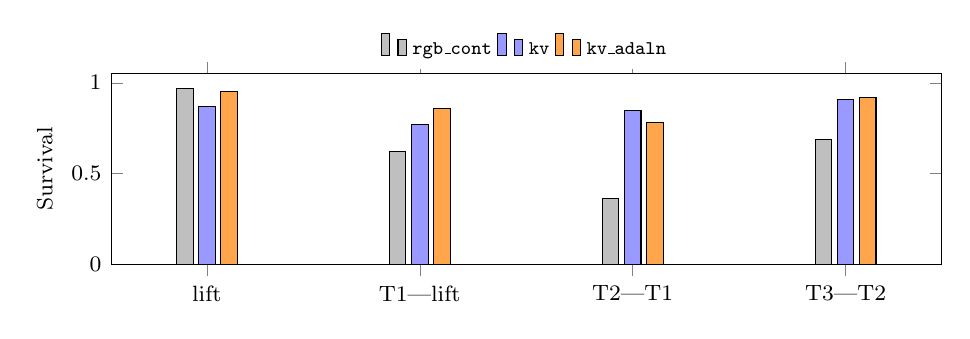
\begin{tikzpicture}
\begin{axis}[
  ybar, bar width=6pt, width=\linewidth, height=4.0cm,
  ymin=0, ymax=1.05, ylabel={Survival}, ylabel style={font=\footnotesize},
  symbolic x coords={lift,T1|lift,T2|T1,T3|T2},
  xtick=data, tick label style={font=\footnotesize},
  legend style={font=\scriptsize, at={(0.5,1.02)}, anchor=south,
    legend columns=3, draw=none},
  enlarge x limits=0.15]
\addplot[fill=gray!50] coordinates {(lift,0.97) (T1|lift,0.62) (T2|T1,0.36) (T3|T2,0.69)};
\addplot[fill=blue!40] coordinates {(lift,0.87) (T1|lift,0.77) (T2|T1,0.85) (T3|T2,0.91)};
\addplot[fill=orange!70] coordinates {(lift,0.95) (T1|lift,0.86) (T2|T1,0.78) (T3|T2,0.92)};
\legend{\arm{rgb\_cont}, \arm{kv}, \arm{kv\_adaln}}
\end{axis}
\end{tikzpicture}
\caption{GR00T stage-wise survival on seen objects, pooled over 3 seeds
$\times$ 20 scenes: lift, then each transfer given the previous one.}
\label{fig:stages}
\end{figure}

\subsection{Robustness and data}
\label{sec:robustness}

\begin{table}[t]
\centering
\caption{GR00T robustness and data size (seen successes of 60).}
\label{tab:robust}
\footnotesize
\setlength{\tabcolsep}{4pt}
\begin{tabular}{@{}lccc@{}}
\toprule
Condition & \arm{rgb\_cont} & \arm{kv} & \arm{kv\_adaln} \\
\midrule
nominal                                  & 9 & 31 & 35 \\
\multicolumn{4}{@{}l}{\textit{entity noise at test time (movable objects)}} \\
\quad 2\,mm, 2$^\circ$                   & -- & 32 & 28 \\
\quad 5\,mm, 2$^\circ$                   & -- & 28 & 33 \\
\quad 10\,mm, 5$^\circ$                  & -- & 24 & 23 \\
\quad 5\,mm, 2$^\circ$, 10\% dropped     & -- & 25 & 24 \\
\quad 5\,mm, 2$^\circ$, 25\% dropped     & -- & 12 & 10 \\
\multicolumn{4}{@{}l}{\textit{unseen textures and lighting}} \\
\quad visual shift                       & 2 & 25 & 24 \\
\multicolumn{4}{@{}l}{\textit{training runs (seen / held-out)}} \\
\quad 19                                 & 2 / 0 & -- & 8 / 4 \\
\quad 38                                 & 4 / 1 & -- & 28 / 15 \\
\quad 75                                 & 9 / 0 & 31 / 7 & 35 / 11 \\
\bottomrule
\end{tabular}
\end{table}

\textbf{Pose noise.} Table~\ref{tab:robust} perturbs the entities of movable
objects at test time. At 2--5\,mm and 2$^\circ$, typical of fiducial
tracking, success is unchanged within seed noise. At 10\,mm and 5$^\circ$ it
falls (\arm{kv\_adaln} 35$\rightarrow$23, $p=0.017$) but stays well above
the control. Dropping a quarter of the object entities brings both arms down
to near the control's level (12 and 10).

\textbf{Visual shift.} Under unseen background textures and random lighting,
the RGB control collapses (9$\rightarrow$2, $p=0.039$). The conditioned arms
keep 25 and 24 successes, and beat the control under shift with $p<0.001$.

\textbf{Data size.} Conditioning beats the budget control at every data size
tried. At 19 runs the gain shows mainly in first transfers on held-out sizes
(7$\rightarrow$22 episodes, $p=0.001$). From 38 runs on it shows in full
successes. Steps were fixed across data sizes, so this supports a benefit at
every size rather than a data-efficiency slope.

% =====================================================================
\section{RQ2: Does Relational Composition Help?}
\label{sec:rq2}

Sec.~\ref{sec:controls} shows that the benefit comes from per-entity
retrieval. It also leaves a precise residual. On ACT, the policy's grasp
misses by \textasciitilde9\,mm horizontally in every arm (8.6--10.7\,mm
against the control's 8.7\,mm), whereas orientation and gripper timing are
correct. With only absolute poses, each mechanism must learn the
gripper-to-object subtraction itself. \arm{kv\_rel} provides it.

\textbf{Arms.} We compare \arm{kv\_rel} with \arm{kv} and two controls built
like those of Table~\ref{tab:controls}:
\begin{itemize}
  \item \arm{kv\_mlp} replaces the pairwise term in~\eqref{eq:rel} with a
    per-entity MLP of equal parameter count, which controls for capacity;
  \item \arm{kv\_rel\_shuf} computes $u_{ij}$ against the entities of
    another training scene while keeping $e_i$ correct, which controls for
    information.
\end{itemize}
A relational gain is claimed only if \arm{kv\_rel} beats both controls on
every seed.

\begin{table}[t]
\centering
\caption{RQ2 on restock, GR00T (successes of 60; median horizontal grasp
error at gripper closure).}
\label{tab:rq2}
\footnotesize
\setlength{\tabcolsep}{4pt}
\begin{tabular}{@{}lcccc@{}}
\toprule
Arm & Seen & Held-out & Novel & Grasp err.\,[mm] \\
\midrule
\arm{rgb\_cont}      & 9    & 0    & \tbd & \tbd \\
\arm{kv}             & 31   & 7    & \tbd & \tbd \\
\arm{kv\_mlp}        & \tbd & \tbd & \tbd & \tbd \\
\arm{kv\_rel\_shuf}  & \tbd & \tbd & \tbd & \tbd \\
\arm{kv\_rel}        & \tbd & \tbd & \tbd & \tbd \\
\arm{kv\_rel}, 2 layers & \tbd & \tbd & \tbd & \tbd \\
\bottomrule
\end{tabular}
\end{table}

\begin{table*}[t]
\centering
\caption{RoboTwin~2.0, GR00T N1.7 and ACT: success rate (\%) over 3
training seeds $\times$ 20 scenes, min--max across seeds in brackets.
Expert: success rate of the scripted expert, the ceiling for each task.}
\label{tab:robotwin-results}
\footnotesize
\setlength{\tabcolsep}{3.5pt}
\begin{tabular}{@{}llccccccc@{}}
\toprule
Backbone & Task & Expert & \arm{rgb\_cont} & \arm{kv} & \arm{kv\_adaln} & \arm{kv\_rel} & \arm{kv}\,+c & \arm{kv\_rel}\,+c \\
\midrule
\multirow{6}{*}{GR00T}
 & Stack Blocks Three    & \tbd & \tbd & \tbd & \tbd & \tbd & \tbd & \tbd \\
 & Blocks Ranking RGB    & \tbd & \tbd & \tbd & \tbd & \tbd & \tbd & \tbd \\
 & Put Bottles Dustbin   & \tbd & \tbd & \tbd & \tbd & \tbd & -- & -- \\
 & Place Cans Plasticbox & \tbd & \tbd & \tbd & \tbd & \tbd & -- & -- \\
 & Place Bread Basket    & \tbd & \tbd & \tbd & \tbd & \tbd & -- & -- \\
 & \textit{Mean}         & \tbd & \tbd & \tbd & \tbd & \tbd & \tbd & \tbd \\
\midrule
\multirow{6}{*}{ACT}
 & Stack Blocks Three    & \tbd & \tbd & \tbd & \tbd & \tbd & \tbd & \tbd \\
 & Blocks Ranking RGB    & \tbd & \tbd & \tbd & \tbd & \tbd & \tbd & \tbd \\
 & Put Bottles Dustbin   & \tbd & \tbd & \tbd & \tbd & \tbd & -- & -- \\
 & Place Cans Plasticbox & \tbd & \tbd & \tbd & \tbd & \tbd & -- & -- \\
 & Place Bread Basket    & \tbd & \tbd & \tbd & \tbd & \tbd & -- & -- \\
 & \textit{Mean}         & \tbd & \tbd & \tbd & \tbd & \tbd & \tbd & \tbd \\
\bottomrule
\end{tabular}
\end{table*}

\textbf{Restock.} Table~\ref{tab:rq2} reports the results. \arm{kv\_rel}
reaches \tbd{} seen and \tbd{} held-out successes, against 31 and 7 for
\arm{kv} ($p=\tbd$). The capacity control reaches \tbd{} and the
information control \tbd{}. The horizontal grasp error changes from
\tbd{}\,mm to \tbd{}\,mm.

\textbf{RoboTwin.} Table~\ref{tab:robotwin-results} reports the results.
Averaged over the five tasks, \arm{kv\_rel} reaches \tbd{}\% against
\tbd{}\% for \arm{kv} and \tbd{}\% for the control. The largest gain is on
\tbd{}, whose goal is \tbd{}.

\textbf{Colour.} On the two colour-defined tasks, geometry-only \arm{kv}
reaches \tbd{}\%, against \tbd{}\% for the control. This is expected: no
geometric entity identifies the red block. Adding colour raises it to
\tbd{}\%, and \tbd{}\% with relations.

% =====================================================================
\section{RQ3: Generalisation Across Object Count}
\label{sec:rq3}

\begin{figure}[t]
\centering
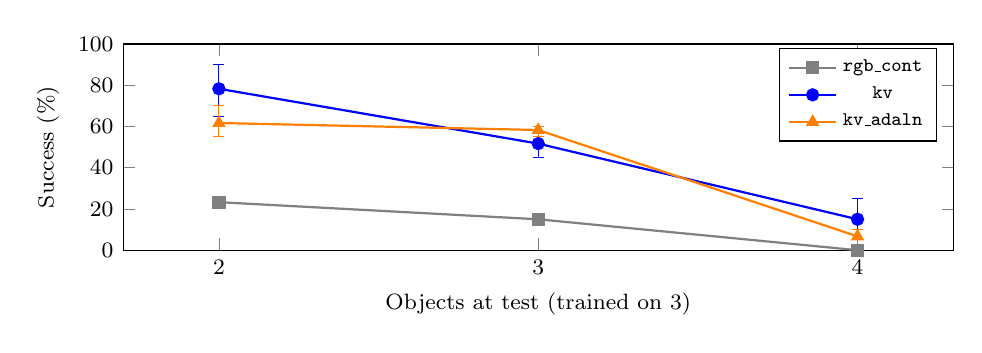
\begin{tikzpicture}
\begin{axis}[
  width=\linewidth, height=4.2cm,
  xmin=1.7, xmax=4.3, xtick={2,3,4}, ymin=0, ymax=100,
  xlabel={Objects at test (trained on 3)}, ylabel={Success (\%)},
  label style={font=\footnotesize}, tick label style={font=\footnotesize},
  legend style={font=\scriptsize, at={(0.98,0.98)}, anchor=north east},
  error bars/y dir=both, error bars/y explicit]
\addplot[gray, mark=square*, thick] coordinates {
  (2,23.3) +- (0,0) (3,15.0) +- (0,0) (4,0.0) +- (0,0)};
\addplot[blue, mark=*, thick, error bars/.cd, y dir=both, y explicit] coordinates {
  (2,78.3) += (0,11.7) -= (0,13.3)
  (3,51.7) += (0,8.3)  -= (0,6.7)
  (4,15.0) += (0,10.0) -= (0,10.0)};
\addplot[orange, mark=triangle*, thick, error bars/.cd, y dir=both, y explicit] coordinates {
  (2,61.7) += (0,8.3) -= (0,6.7)
  (3,58.3) += (0,1.7) -= (0,3.3)
  (4,6.7)  += (0,3.3) -= (0,1.7)};
\legend{\arm{rgb\_cont}, \arm{kv}, \arm{kv\_adaln}}
\end{axis}
\end{tikzpicture}
\caption{GR00T success against object count. Mean over 3 training seeds;
bars span the min--max across seeds. \arm{rgb\_cont} seed ranges are
5--35\%, 10--20\% and 0\%. \textcolor{red}{Add \arm{kv\_rel}.}}
\label{fig:count}
\end{figure}

\begin{table}[t]
\centering
\caption{Trained on three objects. Successes of 60 at 2, 3 and 4 objects;
in brackets, episodes with $\geq$1 transfer at 4 objects.}
\label{tab:rq3}
\footnotesize
\setlength{\tabcolsep}{4pt}
\begin{tabular}{@{}llcccc@{}}
\toprule
& Arm & 2 & 3 & 4 & [4: $\geq$1] \\
\midrule
\multirow{4}{*}{GR00T}
 & \arm{rgb\_cont} & 14 & 9  & 0 & [37] \\
 & \arm{kv}        & \textbf{47} & 31 & \textbf{9} & [31] \\
 & \arm{kv\_adaln} & \textbf{37} & 35 & 4 & [19] \\
 & \arm{kv\_rel}   & \tbd & \tbd & \tbd & [\tbd] \\
\midrule
\multirow{4}{*}{ACT}
 & \arm{rgb\_cont}  & 18 & 21 & 0 & [22] \\
 & \arm{kv}         & 18 & 22 & 0 & [14] \\
 & \arm{kv\_adaln}  & 16 & 22 & 0 & [18] \\
 & \arm{kv\_tokens} & 19 & 26 & 0 & [23] \\
\bottomrule
\end{tabular}
\end{table}

All policies are trained on three objects and evaluated on two and four
(Table~\ref{tab:rq3}, Fig.~\ref{fig:count}).

\textbf{Two objects.} GR00T's conditioning carries over strongly.
\arm{kv} raises success from 14 to 47 of 60 and \arm{kv\_adaln} to 37 (both
$p<0.001$), on every seed (\arm{kv}: 13--18 of 20; control: 1--7).

\textbf{Four objects.} \arm{kv} completes 9 scenes, where the control
completes none ($p=0.004$), on every seed (1--5 of 20). The pooled arm
behaves differently: \arm{kv\_adaln} reaches a first transfer less often
than the control (37$\rightarrow$19, $p=0.002$) and less often than \arm{kv}
(31$\rightarrow$19, $p=0.043$). ACT trained on per-object clips shows the same split
(first transfers 23 for \arm{kv} against 12 for \arm{kv\_adaln}); trained on
continuous runs it does not (Table~\ref{tab:rq3}). A plausible reading, consistent with
Table~\ref{tab:controls}, is that a scene summary fitted on three-object
scenes misleads in a four-object scene, while per-entity retrieval is not
tied to a count. Mean aggregation in~\eqref{eq:rel} is designed to keep that
property. \arm{kv\_rel} reaches \tbd{} of 60 at four objects ($p=\tbd$
against \arm{kv}).

\textbf{ACT.} No ACT policy completes a four-object scene: 0 of 1380
episodes across all arms and training formats, even with the full 800
steps. Since four objects stay inside the training workspace, this is a
limit on sequence length (three transfers is the longest sequence ACT was
trained on) that conditioning does not lift.

% =====================================================================
\section{Discussion and Limitations}
\label{sec:discussion}

\textbf{Why does the benefit depend on the backbone?} ACT trains its whole
network on the demonstrations, and with the extra budget it reaches the
conditioned arms' grasp precision from pixels alone (3D grasp error
17.5$\rightarrow$10.0\,mm from the extra steps, and 9.2--11.9\,mm for the
conditioned arms). GR00T adapts only its action head on a frozen backbone,
so exact object state may substitute for visual precision it never acquires.
On $\pi_{0.5}$ and SmolVLA the branch at matched proportion is small in
absolute terms (\textasciitilde1\,M parameters, against
\textasciitilde150\,M on GR00T). A larger branch, compared against a control
given the same extra capacity, remains to be tested.

\textbf{Limitations.}
\begin{itemize}
  \item \emph{Ground-truth entities.} Entities come from the simulator. The
    noise study indicates that fiducial-level tracking suffices, but no
    perception pipeline is evaluated.
  \item \emph{Simulation only.} All results are in simulation.
    \textcolor{red}{Real-robot validation: add or justify.}
  \item \emph{Restock geometry.} The restock objects differ only in size,
    so ``held-out identity'' means unseen size.
  \item \emph{Unseeded VLA sampling.} The VLA policies sample their initial
    action noise without a fixed seed, so individual scenes do not replay
    exactly. Paired comparisons remain valid, and the seed ranges carry
    this variance.
  \item \emph{Seed variance.} Seed variance is large. A same-recipe
    retraining of one GR00T arm differed from the original at $p=0.008$ on
    one metric, which is why we claim only effects that are consistent
    across seeds.
\end{itemize}

% =====================================================================
\section{Conclusion}
\label{sec:conclusion}
Object-centric state helps a pretrained VLA when it is retrieved per action
query and controlled against equal extra training. On GR00T~N1.7 it
quadruples success on seen objects, enables success on held-out geometry,
and survives visual shift and fiducial-level pose noise. The gain is object
information delivered by query-dependent attention, not capacity and not a
pooled summary. It is not universal: ACT benefits only on held-out geometry,
and $\pi_{0.5}$ and SmolVLA not at matched capacity. Adding explicit
pairwise relations \tbd[ {[}summary of RQ2{]}], and across object count
\tbd[ {[}summary of RQ3{]}]. Future work will replace ground-truth entities
with learned perception and validate on hardware.

% =====================================================================
\begin{thebibliography}{12}

\bibitem{zhao2023act}
T.~Z. Zhao, V.~Kumar, S.~Levine, and C.~Finn, ``Learning fine-grained
bimanual manipulation with low-cost hardware,'' in \emph{Proc. Robot.: Sci.
Syst. (RSS)}, 2023.

\bibitem{bjorck2025gr00t}
J.~Bjorck \emph{et al.}, ``GR00T N1: An open foundation model for generalist
humanoid robots,'' \emph{arXiv:2503.14734}, 2025. % VERIFY; cite N1.7 if a report exists

\bibitem{pi05}
Physical Intelligence \emph{et al.}, ``$\pi_{0.5}$: A vision-language-action
model with open-world generalization,'' \emph{arXiv:2504.16054}, 2025. % VERIFY

\bibitem{shukor2025smolvla}
M.~Shukor \emph{et al.}, ``SmolVLA: A vision-language-action model for
affordable and efficient robotics,'' \emph{arXiv:2506.01844}, 2025. % VERIFY

\bibitem{li2025controlvla}
P.~Li \emph{et al.}, ``ControlVLA: Few-shot object-centric adaptation for
pre-trained vision-language-action models,'' \emph{arXiv:2506.16211}, 2025. % VERIFY authors/venue

\bibitem{lpwm}
\textcolor{red}{Authors}, ``\textcolor{red}{LPWM title},''
\emph{arXiv:2603.04553}, 2026. % VERIFY: placeholder

\bibitem{chen2025robotwin2}
T.~Chen \emph{et al.}, ``RoboTwin 2.0: A scalable data generator and
benchmark with strong domain randomization for robust bimanual robotic
manipulation,'' \emph{arXiv:2506.18088}, 2025. % VERIFY

\bibitem{zhu2022viola}
Y.~Zhu, A.~Joshi, P.~Stone, and Y.~Zhu, ``VIOLA: Imitation learning for
vision-based manipulation with object proposal priors,'' in \emph{Proc.
Conf. Robot Learn. (CoRL)}, 2022.

\bibitem{locatello2020slot}
F.~Locatello \emph{et al.}, ``Object-centric learning with slot attention,''
in \emph{Proc. Adv. Neural Inf. Process. Syst. (NeurIPS)}, 2020.

\bibitem{santoro2017rn}
A.~Santoro \emph{et al.}, ``A simple neural network module for relational
reasoning,'' in \emph{Proc. Adv. Neural Inf. Process. Syst. (NeurIPS)}, 2017.

\bibitem{battaglia2018relational}
P.~W. Battaglia \emph{et al.}, ``Relational inductive biases, deep learning,
and graph networks,'' \emph{arXiv:1806.01261}, 2018.

\bibitem{zaheer2017deepsets}
M.~Zaheer \emph{et al.}, ``Deep sets,'' in \emph{Proc. Adv. Neural Inf.
Process. Syst. (NeurIPS)}, 2017.

\end{thebibliography}

\end{document}
